\documentclass[a4paper, 10pt]{article}

\usepackage[slovene]{babel}
\usepackage[utf8]{inputenc}
\usepackage[T1]{fontenc}
\usepackage{lmodern}
\usepackage{amsmath}
\usepackage{amsfonts}
\usepackage{amssymb}
\usepackage{enumitem}
\usepackage{epsdice}
\usepackage{array}
\usepackage[table]{xcolor}
\usepackage{makecell}
\usepackage{hyperref}

\newcolumntype{P}[1]{>{\centering\arraybackslash}p{#1}}

\begin{document}

\title{\textbf{\LARGE{Kratko poročilo}}}
\author{Karolina Šavli}
\date{5.\ 4.\ 2024}

\maketitle

% =======================================================================================================================

\noindent V projektni nalogi bom pod mentorstvom GEN-I analizirala in napovedovala odjem električne energije 
\textbf{gospodinjskih odjemalcev} (v analizo niso vključeni samooskrbni odjemalci, torej tisti, 
ki imajo lastno sončno elektrarno). Obravnavala bom časovno vrsto; odjem električne energije skozi čas. \\

\noindent Glavni cilj projekta je sestaviti metodo, model, ki bo napovedal odjem za celotni naslednji dan (za naslednjih 24 ur), 
kjer se bodo upoštevali dejavniki, ki se nam zdijo pomembni za napoved (temperatura, sevanje). \\

\noindent Podjetje GEN-I je pripravilo tabelo podatkov, sestavljeno iz sedmih stolpcev:
\begin{itemize}
    \item  \texttt{DateTimeStartUTC}: univerzalni koordinirani čas,
    \item  \texttt{DateTimeStartCET}: srednjeevropski čas,
    \item  \texttt{Odjem ACT}: neto odjem električne energije v kWh,
    \item  \texttt{Temperatura ACT}: dejanska temperatura, 
    \item  \texttt{Temperatura FC}: napovedana temperatura,
    \item  \texttt{Sevanje ACT}: dejansko sevanje in
    \item  \texttt{Sevanje FC}: napovedano sevanje. 
\end{itemize}

\begin{figure}[h!]
    \centering
    \caption{Podatki, 2021-2024 (vir: GEN-I)}\par\medskip
    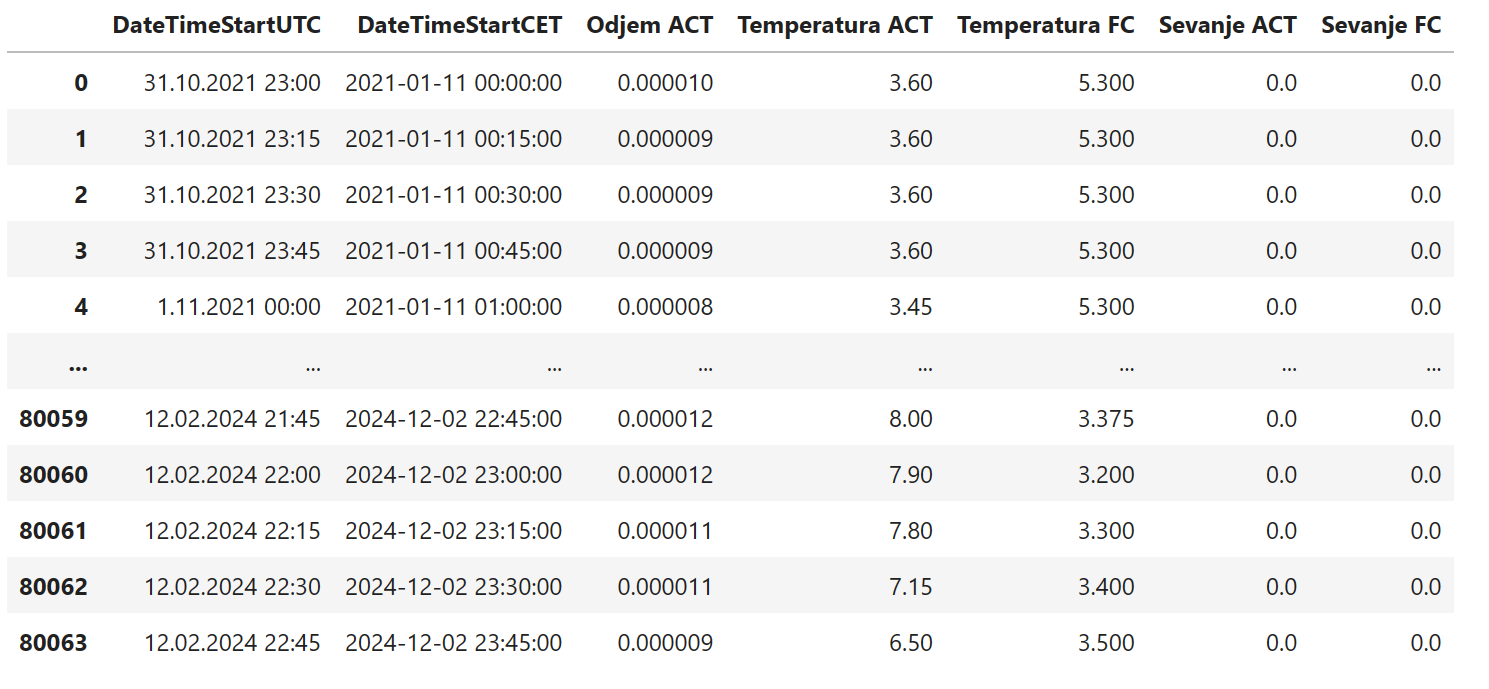
\includegraphics[width=\textwidth]{tabela.png}
\end{figure}

\noindent Uporabljala bom vse stolpce v tabeli, razen stolpca \texttt{DateTimeStartUTC}, saj v 
okviru časa ključen stolpec \texttt{DateTimeStartCET}.  \\

\noindent Odjem je podan za odboje od $1.~\text{novembra}~2021$ 
do $12.~\text{februarja}~2024$,
na vsakih $15$ minut in obsega $80063$ enot podatkov. \\

\subsection*{Motivacija}

\noindent Poglejmo si odjem za leti $2022$ in $2023$. Zaradi boljše preglednosti 
so podatki povprečeni na dnevni ravni.

\begin{figure}[h!]
    \centering
    \caption{Odjem električne energije, 2022-2023}\par\medskip
    \label{fig:LineGraf}
    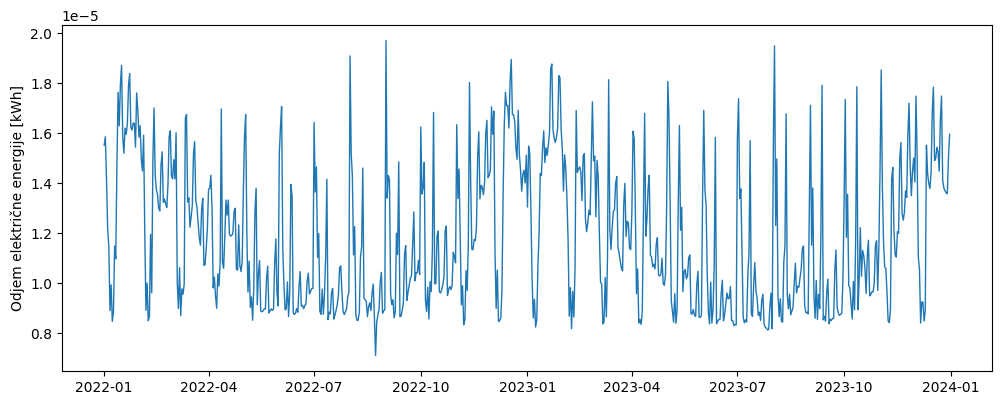
\includegraphics[width=0.95\textwidth]{output.png}
\end{figure}

\noindent S Slike~\ref{fig:LineGraf} je razvidna sezonskost - očitno večji odjem v zimskih mesecih - kar je pomembno pri 
načrtovanju in upravljanju proizvodnje in distribucije električne energije. 
V zimskih mesecih je odjem višji, zaradi ogrevanja, razsvetljave, saj se število ur 
dnevne svetlobe podaljša in nasploh se poveča uporaba električnih aparatov, kot 
so grelniki in sušilniki.  \\

\begin{figure}[h!]
    \centering
    \caption{Povezava med odjemom in temperaturo ter sevanjem, 2021-2024}\par\medskip
    \label{fig:Scatter}
    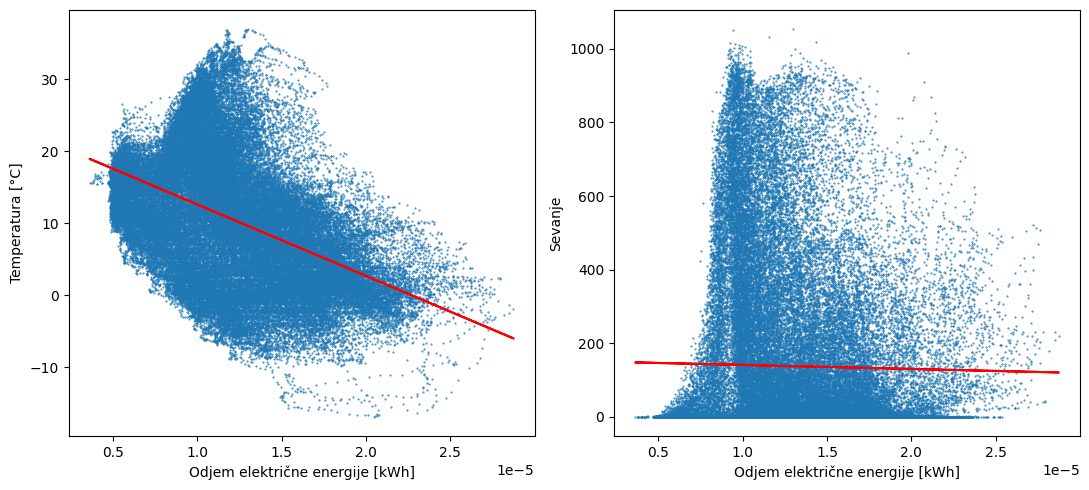
\includegraphics[width=0.95\textwidth]{output_dva.png}
\end{figure}

\noindent Torej na odjem električne energije ključno vpliva del leta in s tem temperature, kar je razvidno tudi iz Slike~\ref{fig:Scatter}.  
V tabeli pa imamo podane tudi podatek 
sevanja, ki pričakujem, da ne bo tako pomemben, saj v moji analizi niso 
vključeni odjemalci, ki imajo sončno elektrarno. S Slike~\ref{fig:Scatter} res ni 
opaziti povezave med odjemom in sevanjem. 
Mogoče pa bo vseeno sevanje
imelo nekaj vpliva pri napovedovanju, saj močna sončna svetloba vendarle povzroči povečano porabo 
električne energije, saj se poveča uporaba naprav za hlajenje. \\
Podatek sevanja je ključen predvsem v primeru obravnave samooskrbnih odjemalcev, ki
jih moja analiza ne vključuje. \\

\noindent Analiza in napovedovanje bo v večini izvedeno v programskem jeziku Python, na zgornjih podatki, ki jih bom 
mogoče dopolnila s kakšnin novim, relevantnim dejavnikom za napoved, ki ga bom najverjetneje pridobila
s strani \href{https://ot.borzen.si/Domov/Podatki-trga/Koli%C4%8Dine-in-zneski-izravnave}{Borzen}. \\


\end{document}